% Created 2022-11-03 Thu 09:47
% Intended LaTeX compiler: pdflatex
\documentclass[bigger]{beamer}
\usepackage[utf8]{inputenc}
\usepackage[T1]{fontenc}
\usepackage{graphicx}
\usepackage{grffile}
\usepackage{longtable}
\usepackage{wrapfig}
\usepackage{rotating}
\usepackage[normalem]{ulem}
\usepackage{amsmath}
\usepackage{textcomp}
\usepackage{amssymb}
\usepackage{capt-of}
\usepackage{hyperref}
\usetheme{Madrid}
\author{Fernando Zhapa-Camacho}
\date{\textit{<2022-11-03 Thu>}}
\title{Categorical representation of OWL ontologies}
\hypersetup{
 pdfauthor={Fernando Zhapa-Camacho},
 pdftitle={Categorical representation of OWL ontologies},
 pdfkeywords={},
 pdfsubject={},
 pdfcreator={Emacs 27.1 (Org mode 9.3)}, 
 pdflang={English}}
\begin{document}

\maketitle
\begin{frame}{Outline}
\tableofcontents
\end{frame}




\section{Introduction}
\label{sec:orgd1839e3}

\begin{frame}[label={sec:orge04952a}]{Motivation}
\begin{itemize}
\item OWL ontologies represent complex domain knowledge
\item Representing semantics on OWL ontologies is useful for tasks such as ontology aligment, link prediction (in KG), etc.
\end{itemize}
\end{frame}


\section{Method}
\label{sec:orga884438}

\begin{frame}[label={sec:org10f9ca8}]{Category Theory}
\begin{columns}
\begin{column}{0.5\columnwidth}
\centering
\(C \sqcap D\)

\begin{figure}[htbp]
\centering
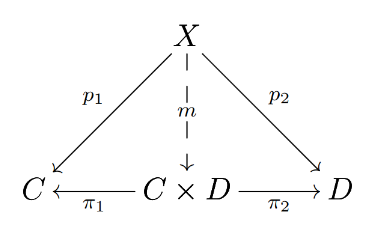
\includegraphics[width=.9\linewidth]{imgs/product.png}
\caption{\label{fig:org7a558ef}Categorical product}
\end{figure}
\end{column}

\begin{column}{0.5\columnwidth}
\centering
\(C \sqcup D\)
\begin{figure}[htbp]
\centering
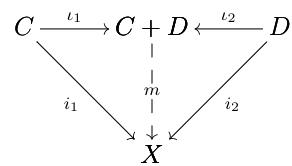
\includegraphics[width=.9\linewidth]{imgs/coproduct.png}
\caption{\label{fig:orgf585a4a}Categorical coproduct}
\end{figure}
\end{column}
\end{columns}
\end{frame}

\section{Experimental setup}
\label{sec:org7b598a4}


\begin{frame}[label={sec:org1028660}]{Methodology}
\begin{itemize}
\item OWL2Vec* projection method (no literals)
\item Graph based on categorical diagrams

\item Random walks over graphs
\end{itemize}
\end{frame}

\begin{frame}[label={sec:orgf43fe29}]{Example: \(C \sqsubseteq \exists R. D\)}
\begin{itemize}
\item \(C \sqsubseteq \Phi\)
\item \(C \sqsubseteq \exists R. D\)
\item \(\forall x (C(x) \to \exists y(R(x,y) \land D(y)))\)
\end{itemize}




\begin{columns}
\begin{column}{0.5\columnwidth}
\begin{figure}[htbp]
\centering
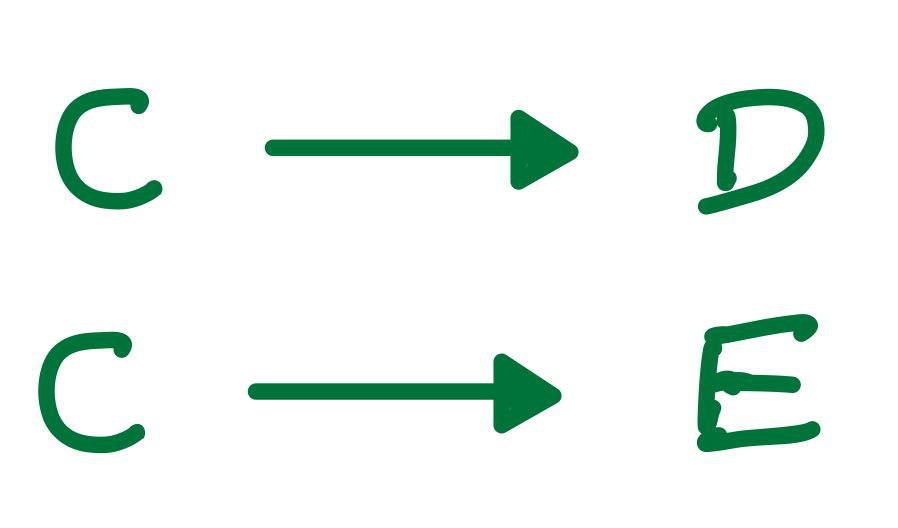
\includegraphics[height=2cm]{imgs/owl2vec1.jpg}
\caption{\label{fig:org8bf5cf9}OWL2Vec*}
\end{figure}
\end{column}

\begin{column}{0.5\columnwidth}
\begin{figure}[htbp]
\centering
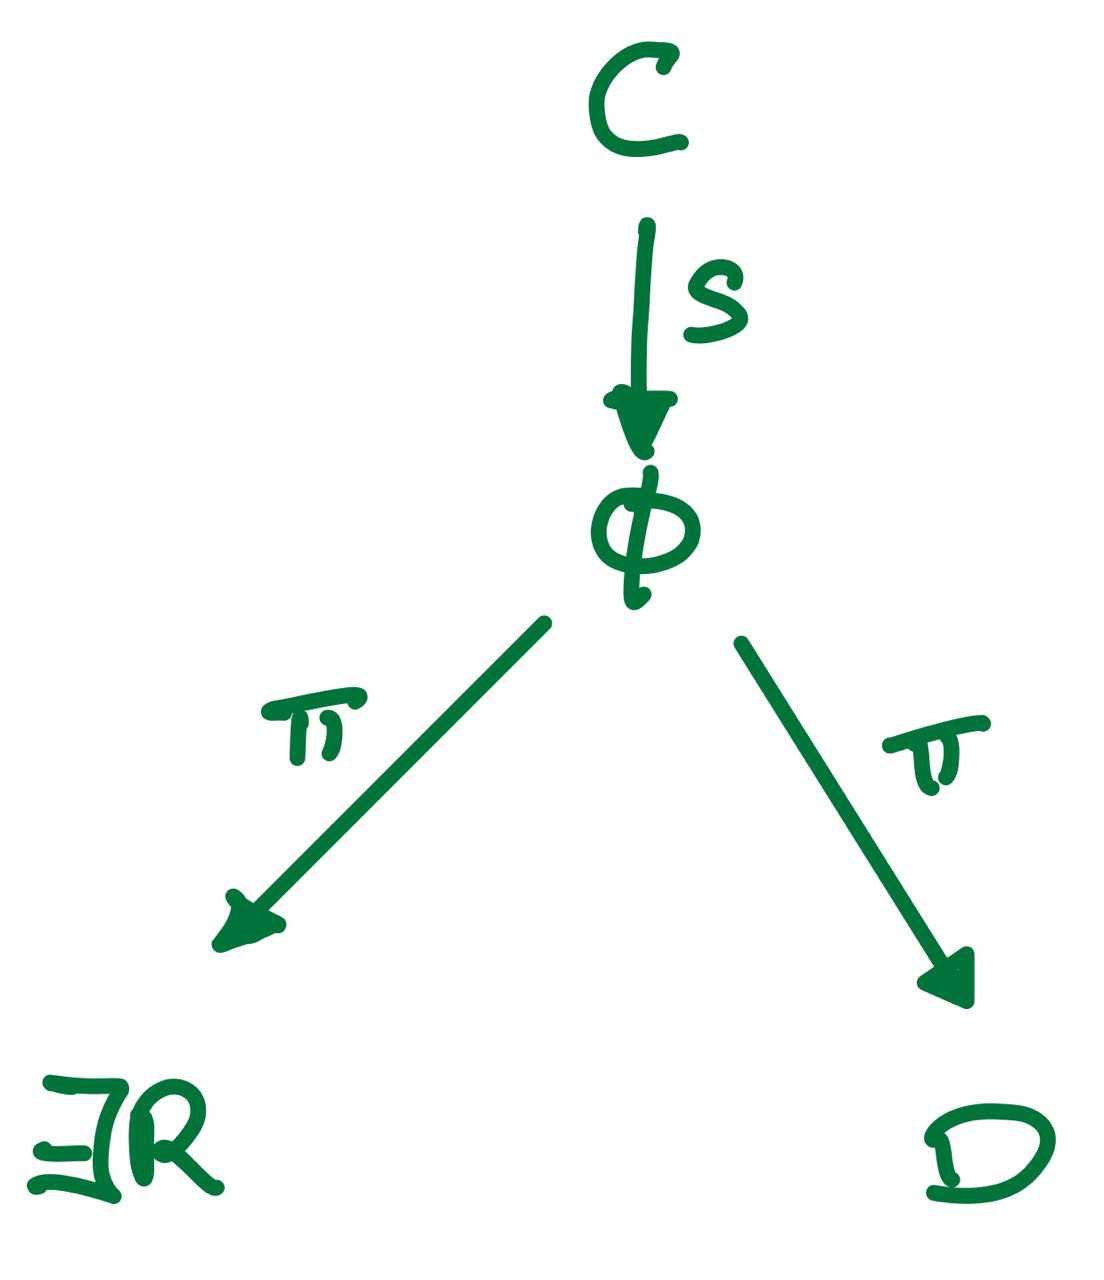
\includegraphics[height=4cm]{imgs/cat1.jpg}
\caption{\label{fig:orga93999a}Categorical}
\end{figure}
\end{column}
\end{columns}
\end{frame}

\begin{frame}[label={sec:orgcde4b2f}]{Example: \(C \sqsubseteq \exists R. D\)}
\begin{itemize}
\item \(C \sqsubseteq \Phi\)
\item \(C \sqsubseteq \forall R. D\)
\item \(\forall x (C(x) \to \forall y (R(x,y) \to D(y)))\)
\item \(\forall x (C(x) \to \forall y ( \lnot R(x,y) \lor D(y)))\)
\end{itemize}

\begin{columns}
\begin{column}{0.5\columnwidth}
\begin{figure}[htbp]
\centering
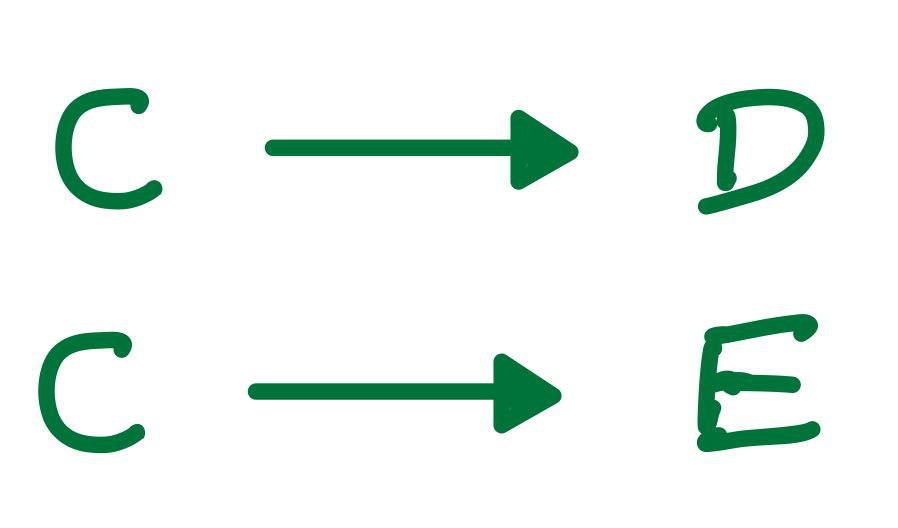
\includegraphics[height=2cm]{imgs/owl2vec1.jpg}
\caption{\label{fig:orgd798a4c}OWL2Vec*}
\end{figure}  
\end{column}

\begin{column}{0.5\columnwidth}
\begin{figure}[htbp]
\centering
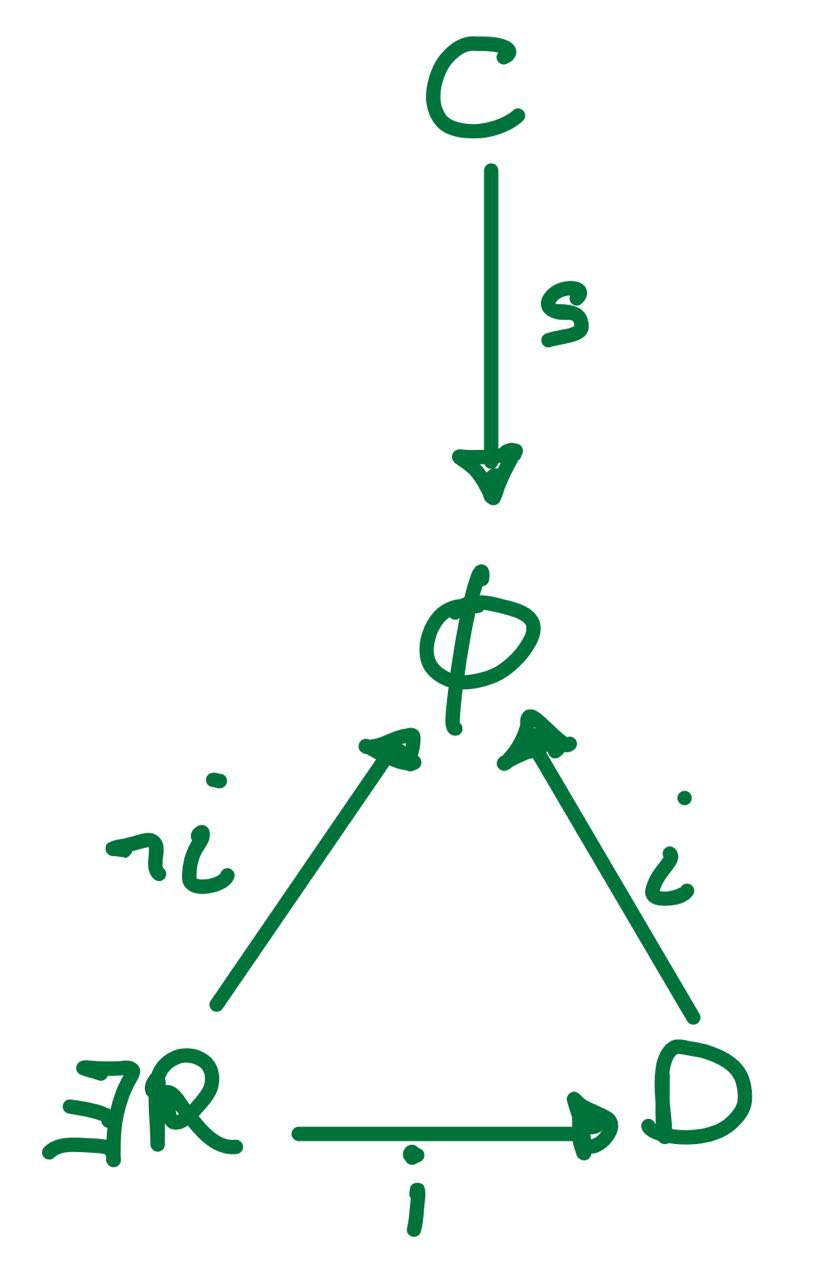
\includegraphics[height=4cm]{imgs/cat2.jpg}
\caption{\label{fig:orgb83d846}Categorical}
\end{figure}
\end{column}
\end{columns}
\end{frame}



\begin{frame}[label={sec:org8abfe29}]{Datasets:}
\begin{itemize}
\item Gene Ontology (subsumption test: \(C \sqsubseteq D\))
\item Food Ontology (subsumption test: \(C \sqsubseteq D\))
\item HeLis Ontology (membership test: \(C(a)\))
\end{itemize}
\end{frame}


\begin{frame}[label={sec:org34e5cf6}]{Connected components on projected graphs}
\begin{columns}
\begin{column}{0.33\columnwidth}
\alert{Gene Ontology}

\begin{itemize}
\item OWL2Vec*: 275
\item Categorical: 239
\end{itemize}
\end{column}

\begin{column}{0.33\columnwidth}
\alert{Food Ontology}

\begin{itemize}
\item OWL2Vec*: 719
\item Categorical: 559
\end{itemize}
\end{column}

\begin{column}{0.33\columnwidth}
\alert{HeLis Ontology}
\begin{itemize}
\item OWL2Vec*: 6
\item Categorical: 8
\end{itemize}
\end{column}
\end{columns}
\end{frame}


\section{Results}
\label{sec:org38f6c8d}

\begin{frame}[label={sec:org5706012}]{Embedding the graph using random walks}
\begin{center}
\begin{tabular}{lllll}
 &  & FoodOn &  & \\
\hline
 & Hits@1 & Hits@5 & Hits@10 & MRR\\
\hline
OWL2Vec* & 0.001935 & 0.008018 & \alert{0.031241} & 0.009610\\
Categorical & \alert{0.010738} & \alert{0.011564} & 0.011564 & \alert{0.012318}\\
 &  &  &  & \\
\end{tabular}
\end{center}
\end{frame}

\begin{frame}[label={sec:org6eae395}]{Embedding the graph using random walks}
\begin{center}
\begin{tabular}{lllll}
 &  & HeLis &  & \\
\hline
 & Hits@1 & Hits@5 & Hits@10 & MRR\\
\hline
OWL2Vec* & 0.069653 & 0.154073 & 0.220034 & 0.126230\\
Categorical & \alert{0.073852} & \alert{0.185282} & \alert{0.285230} & \alert{0.151987}\\
\end{tabular}
\end{center}
\end{frame}

\begin{frame}[label={sec:orgdbd4831}]{Embedding the graph using random walks}
\begin{center}
\begin{tabular}{lllll}
\hline
 &  & GO &  & \\
\hline
 & Hits@1 & Hits@5 & Hits@10 & MRR\\
\hline
OWL2Vec* & 0.001513 & \alert{0.003868} & \alert{0.005129} & 0.003230\\
Categorical & \alert{0.001766} & 0.003700 & 0.004793 & \alert{0.003485}\\
\hline
\end{tabular}
\end{center}
\end{frame}

\section{Conclusion}
\label{sec:orgf8178ac}

\begin{frame}[label={sec:orgb6a73b3}]{Conclusion}
\begin{itemize}
\item Graph based on CT captures more complex axioms and
\item Is able to differentiate among different operators (\(\forall\), \(\exists\), \ldots{})
\end{itemize}
\end{frame}

\begin{frame}[label={sec:orgec0a86e}]{What's next?}
\begin{itemize}
\item Analyze integration of lexical embeddings
\end{itemize}
\end{frame}

\begin{frame}[label={sec:org5cff5d7}]{}
\centering
\LARGE Thank you
\end{frame}
\end{document}